
\documentclass[a4paper,12pt]{report}
\usepackage[utf8]{inputenc}
\usepackage{graphicx}
\usepackage{cite}
\usepackage{listings}
\usepackage{xcolor}
\usepackage{hyperref}
\usepackage{float}

% Definire un nuovo colore verde scuro
\definecolor{darkgreen}{rgb}{0,0.5,0}

\lstset{
    basicstyle=\ttfamily\small,  % Cambia \footnotesize con la dimensione desiderata (es. \small, \large)
    basicstyle=\ttfamily,
    keywordstyle=\color{blue},
    commentstyle=\color{darkgreen},
    stringstyle=\color{red},
    numbers=left,
    numberstyle=\tiny\color{gray},
    stepnumber=1,
    numbersep=10pt,
    backgroundcolor=\color{white},
    showspaces=false,
    showstringspaces=false,
    showtabs=false,
    frame=single,
    tabsize=2,
    captionpos=b,
    breaklines=true,
    breakatwhitespace=false,
    escapeinside={\%*}{*)}
}

% Per il titolo
\title{Titolo della Tesi}
\author{Nome dell'Autore}
\date{Anno Accademico 2023/2024}

% Inizio del documento
\begin{document}

% Pagina del titolo
\begin{titlepage}
    \begin{center}
        
\includegraphics[width=0.15\textwidth]{units_sigillo.png} 
        \vspace{1cm}
        
        \textsc{\LARGE Università degli studi di Trieste}\\[1.5cm]
        
        \textsc{\Large Dipartimento di Matematica e Geoscienze}\\[0.5cm]
        
        \textsc{\large Intelligenza Artificiale e Data Science}\\[0.5cm]
        
        \vspace{2cm}
        
        % Titolo
        \HRule \\[0.4cm]
        { \huge \bfseries Musica Genetica \\[0.4cm] }
        \HRule \\[1.5cm]
        
        \vspace{2cm}
        
        \begin{minipage}{0.4\textwidth}
            \begin{flushleft} \large
                \emph{Autore:}\\
                Leonardo Angellotti
            \end{flushleft}
        \end{minipage}
        \begin{minipage}{0.4\textwidth}
            \begin{flushright} \large
                \emph{Relatore:} \\
                Luca Manzoni
            \end{flushright}
        \end{minipage}
        
        \vfill
        
        {\large Anno Accademico 2023/2024}
        
    \end{center}
\end{titlepage}

\tableofcontents

\chapter{Introduzione}

\begin{quote}
\centering

C’è una grande differenza tra \textit{impossibile} e \textit{difficile da immaginare}. \\
Il primo riguarda il problema; il secondo riguarda te.

\end{quote}

La Musica Algoritmica ha una lunga storia nell'era pre-informatica, dai lavori 'processuali' di \href{https://youtu.be/UT5lgaE-qZY}{George Brecht (Drip Music, 1962)}, \href{https://youtu.be/pxs35GrZVAs}{Stockhausen (Setz die Segel zur Sonn, 1970)}, \href{https://youtu.be/SZazYFchLRI}{Xenakis (Metastaseis, 1971)} fino a \href{https://youtu.be/o9UsLbsdA6s}{George Lewis (Voyager, 1993)}, ecc. \\

Gli algoritmi di Intelligenza Artificiale (AI) sono una delle tecnologie più ampiamente utilizzate e potenti del ventunesimo secolo. Sebbene la definizione esatta di AI si sia costantemente evoluta, dagli anni '50 di Alan Turing, alle attuali architetture di Deep Learning come Alpha Go, 
rimane fisso il fatto che i correnti modelli di AI per attività creative, sono attualmente agli inizi, e seguono quasi esclusivamente il modello imitato dal dataset su cui sono addestrati. \\
Un altro limite è \textit{filosofico}, infatti l'approccio adottato da tali modelli pone il processo creativo come fosse un problema di ottimizzazione (e non come nell'uomo, la necessita dell'artista a creare). \\ 

esistono comunque esempi musicali che riflettono una certa simmetria e regolarità, facendo riferimento a regole ben precise, come i \href{https://youtu.be/QiBM7-5hA6o}{corali di Bach (Deep Bach)}, la \href{https://folkrnn.org}{Modellazione della Musica Popolare (Folk RNN)}. \\
\\
Modellare la musica è un problema difficile per due ragioni principali: \\
\\
Le gerarchie semantiche sono complesse, soggettive e operano su più scale temporali (dell'ordine di secondi a diversi minuti); \\
\\
Le rappresentazioni audio a frequenze di campionamento dell'udito umano, rendono le sequenze da modellare davvero lunghe, ovvero una tipica canzone di 4 minuti in qualità CD (44 kHz, 16-bit) contiene oltre 10 milioni di timesteps. \\
\\
Un campo di ricerca si è mosso verso la modellizzazione della musica partendo dalle rappresentazioni d'onda.
\href{https://magenta.tensorflow.org }{Magenta di Google} (2016 - 2020), \href{https://openai.com/index/musenet/}{MuseNet di OpenAI} (2019), \href{https://www.flow-machines.com}{Flow Machines di Sony CSL} (2012), il \href{https://ai.meta.com/research/publications/a-universal-music-translation-network/}{Universal Music Translator di Facebook AI Research} (2019) e \href{https://aws.amazon.com/it/deepcomposer/}{Deep Composer di Amazon} (2019)
sono alcuni degli sforzi delle grandi aziende tecnologiche che possono far ricorso ad ampi dataset per il training dei modelli. \\ 
\\
Tuttavia i metodi attuali risultano \textit{rigidi} e la generazione dipende fortemente l'architettura fissata al momento dell'addestramento. \\
(Una rete neurale allenata da un dataset di canzoni pop, non è in grado di generare una melodia blues) \\
\\
\textbf{Struttura della tesi} \\
\\
Nella testi vengono riportate inizialmente le nozioni di base utili alla comprensione degli argomenti trattati. \\
Vengono poi discussi i principali metodi di generazione musicale correnti, e gli studi associati. \\
Infine viene presentato un algoritmo genetico, per la generazione di una sequenza musicale, discutendone i risultati conseguiti. \\
Nelle conclusioni vengono raccolti i traguardi raggiunti, e le limitazioni da superare, nella costruzione algoritmica di nuovi modelli. \\

\chapter{Nozioni di Base}

\section{nozioni algoritmiche}

\subsection{fitness-function}

La fitness function fornisce un punteggio numerico che rappresenta l'efficacia di una soluzione candidata. \\
Questo punteggio guida l'algoritmo nel processo di selezione e ottimizzazione. \\
L'obiettivo è massimizzare o minimizzare la fitness function, a seconda del problema. \\
Negli algoritmi genetici, le soluzioni con punteggi di fitness più alti (genitori) hanno una probabilità maggiore di essere selezionate per la riproduzione e la generazione di nuove soluzioni (prole).

\subsection{modello markoviano}

In un modello markoviano un nuovo stato dipende esclusivamente dallo stato corrente, senza tener conto degli stati passati. \\
Formalmente, questa proprietà si esprime come: 

% Inserimento di un'immagine
\begin{figure}[H]
    \centering
    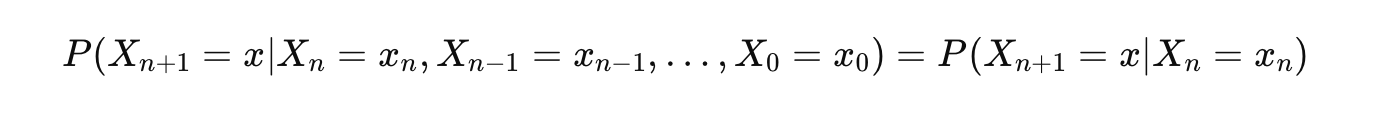
\includegraphics[width=1\textwidth]{/Users/leonardoangellotti/Desktop/tesi latex/immagini/markov1} 
    \label{fig:immagine}
\end{figure}
\\
dove $X_i$ rappresenta lo stato del sistema al tempo $i$. \\
Il modello è costituito da un insieme finito o numerabile di stati. Le transizioni tra stati sono governate da probabilità di transizione che possono essere rappresentate in una matrice. \\
Per una catena di Markov con N stati, la matrice di transizione P è una matrice N×N dove l'elemento $P_ij$ rappresenta la probabilità di transizione dallo stato $i$ allo stato $j$. \\
Le righe della matrice devono sommare a 1: 

% Inserimento di un'immagine
\begin{figure}[H]
    \centering
    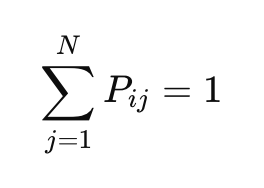
\includegraphics[width=0.2\textwidth]{/Users/leonardoangellotti/Desktop/tesi latex/immagini/markov2} 
    \label{fig:immagine}
\end{figure}

Un modello markoviano può raggiungere una distribuzione stazionaria, dove le probabilità di occupazione degli stati non cambiano più nel tempo. \\
Questo accade quando il sistema raggiunge un equilibrio. \\
Nel caso specifico della tesi questo approccio è adottato per generare una consecuzione di note e accordi.

\subsection{artificial neural network}

Una Artificial Neural Network (ANN), o rete neurale artificiale, è un modello computazionale ispirato alla struttura e al funzionamento del cervello umano, progettato per riconoscere schemi complessi e prendere decisioni basate su input di dati. \\
Le ANNs sono particolarmente utili in vari campi dell'intelligenza artificiale, come il riconoscimento di immagini, il riconoscimento vocale, l'elaborazione del linguaggio naturale e molti altri. \\
\\
\textbf{Funzionamento di una ANN} \\
\\
\textbf{Forward Propagation}: gli input vengono trasmessi attraverso i vari strati della rete, moltiplicando i valori in input per i pesi delle connessioni e applicando una funzione di attivazione. Questo processo persegue fino a raggiungere il livello di output, producendo una previsione.
\\
\textbf{Backward Propagation}: l'errore tra la previsione e il valore reale viene calcolato e usato dalla rete per aggiornare i pesi. Viene usato il calcolo del gradiente per minimizzare l'errore, adattando i pesi in modo iterativo.

\section{nozioni musicali}

% Inserimento di un'immagine
\begin{figure}[H]
    \centering
    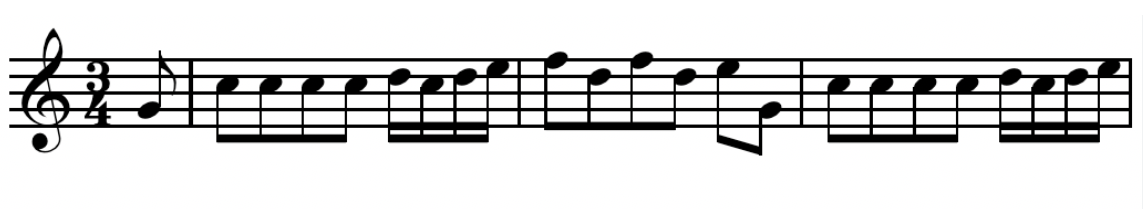
\includegraphics[width=1\textwidth]{/Users/leonardoangellotti/Desktop/tesi latex/immagini/music phrase} 
    \caption{generica linea melodica di uno spartito}
    \label{fig:immagine}
\end{figure}

\subsection{Caratteristiche di una Nota Musicale}

\textbf{Altezza (Pitch):} \\
L'altezza di una nota è la frequenza del suono che produce, determinando quanto sia acuto o grave. \\
Le note sono rappresentate su un pentagramma, dove la posizione verticale della nota indica la sua altezza. \\
Ad esempio, le note su righe o spazi più alti sul pentagramma hanno altezze maggiori. \\
Le note musicali fondamentali nell'ottava sono Do, Re, Mi, Fa, Sol, La, Si. \\
\\
\textbf{Durata:}\\
La durata di una nota indica per quanto tempo viene suonata. \\
\\
Di seguito un'immagine esemplificativa:

% Inserimento di un'immagine
\begin{figure}[H]
    \centering
    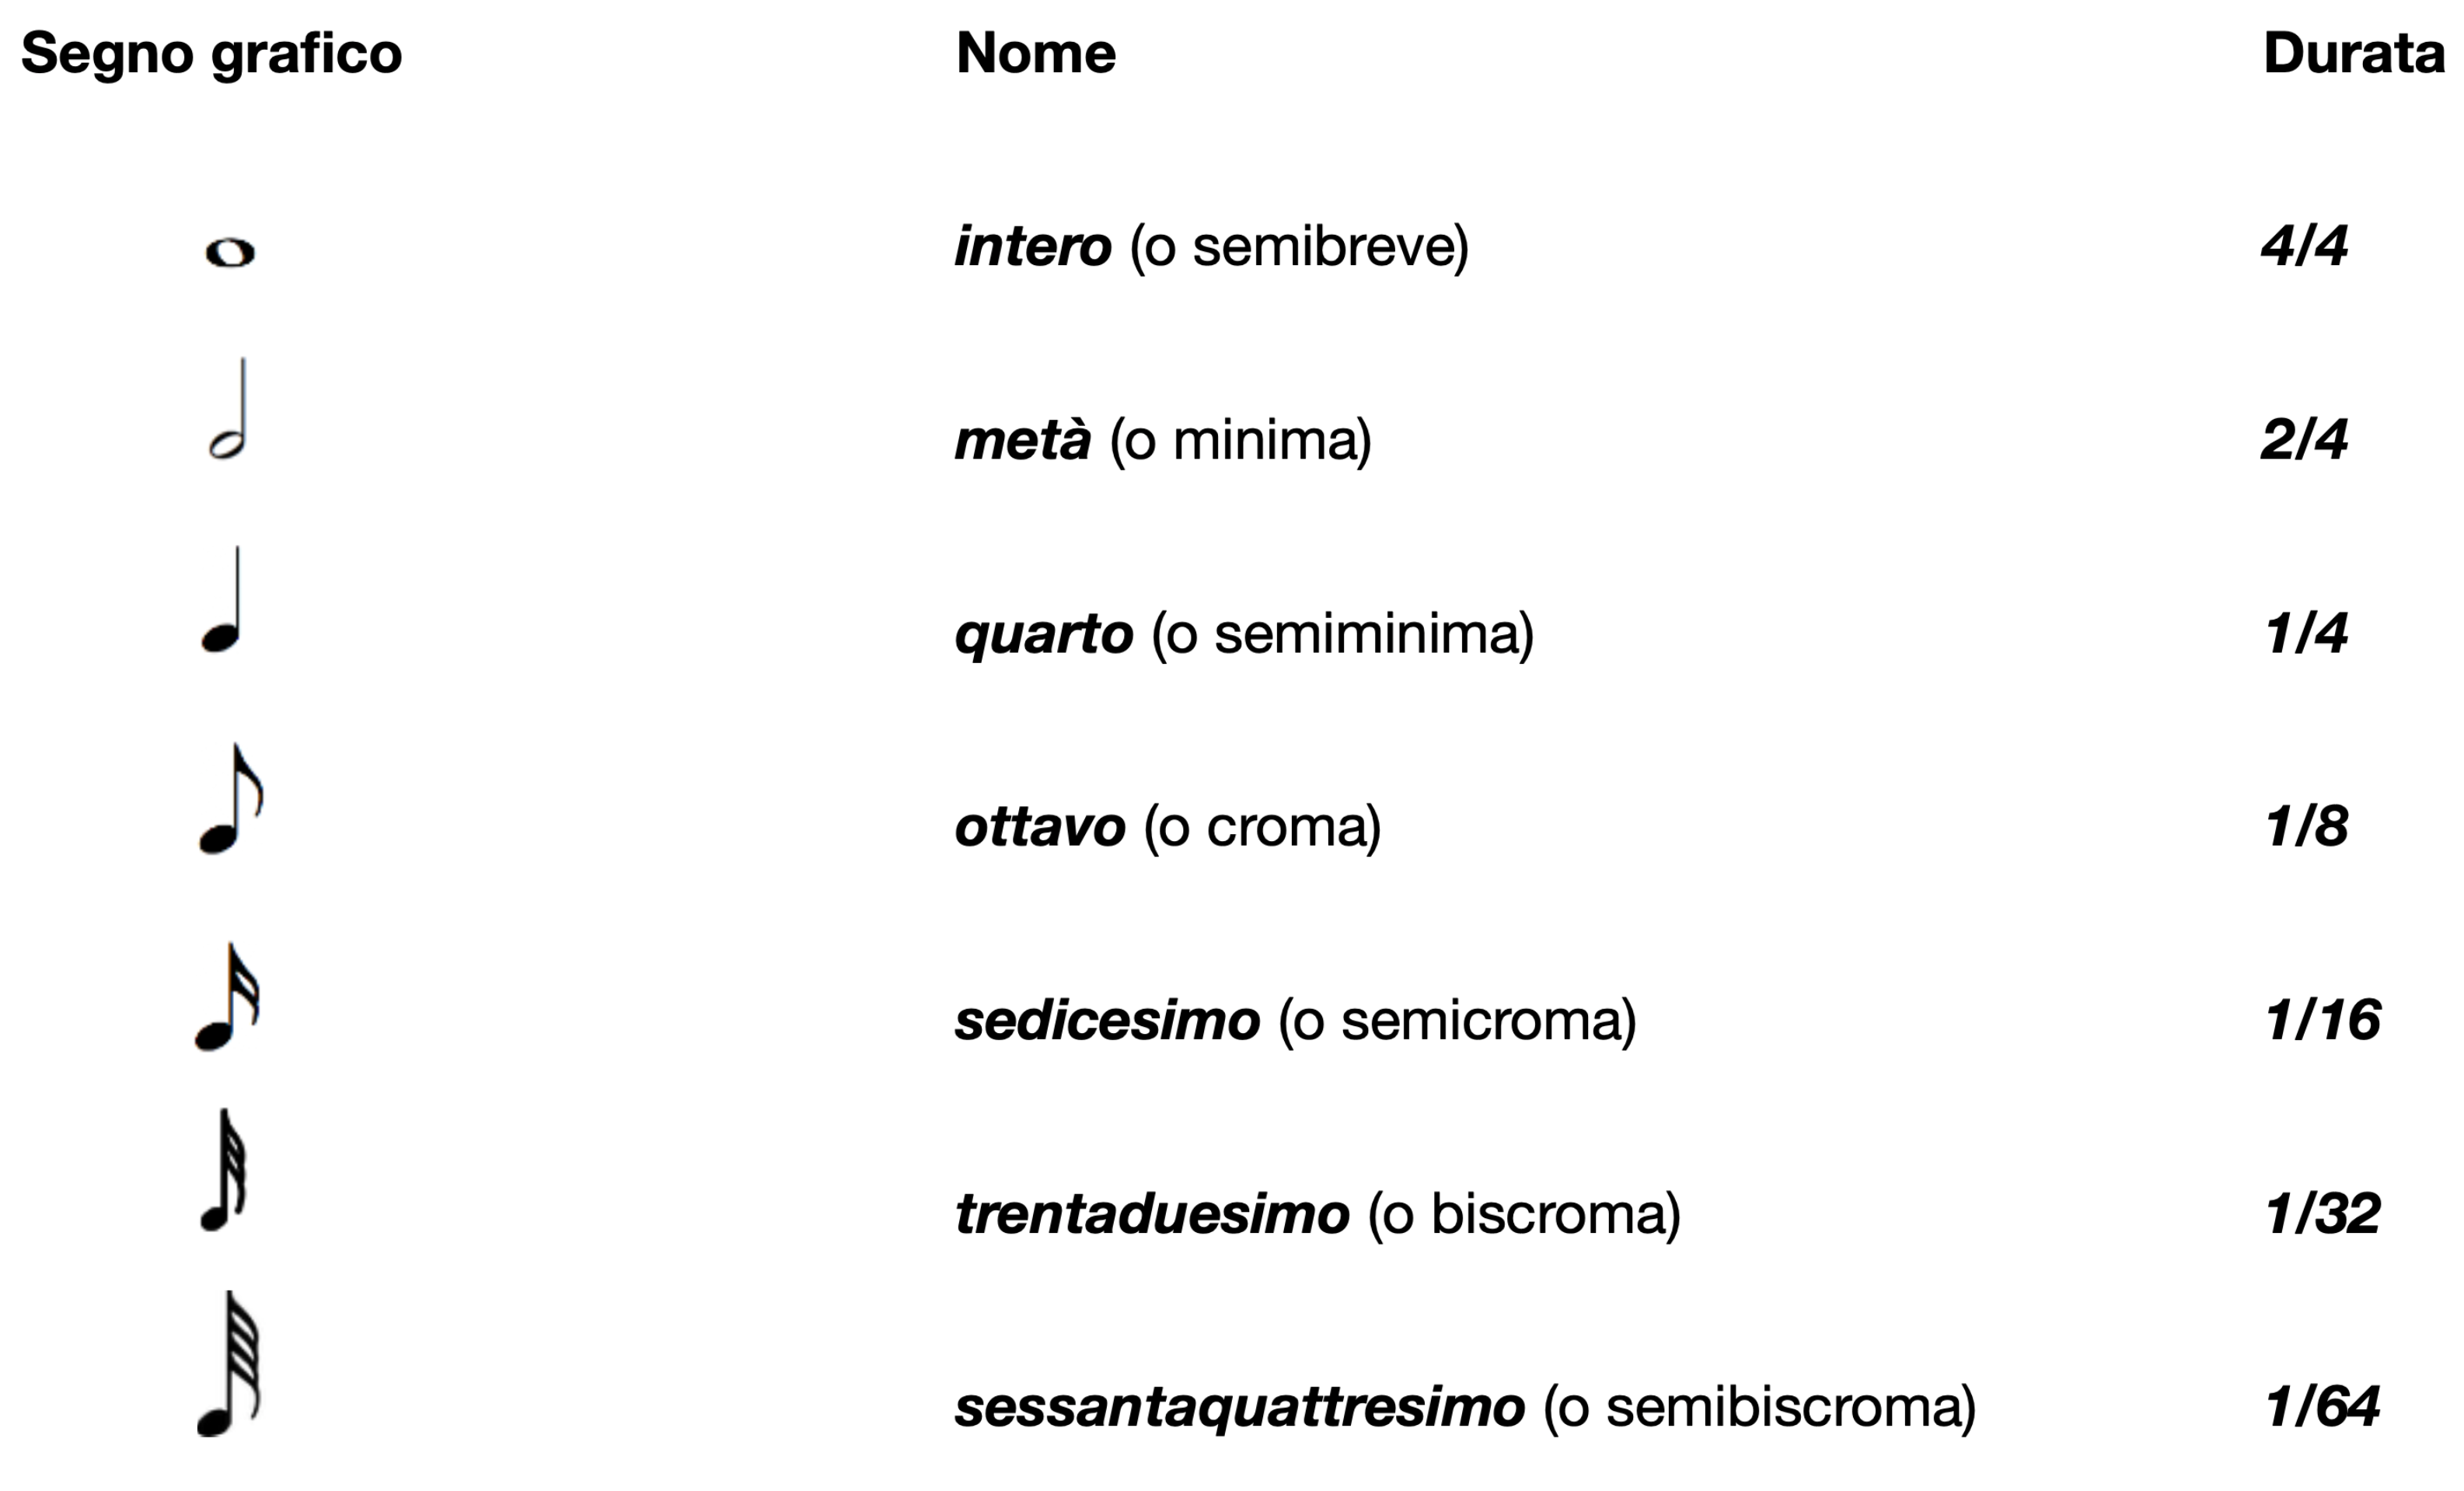
\includegraphics[width=1\textwidth]{/Users/leonardoangellotti/Desktop/tesi latex/immagini/note duration} 
    \caption{tabella riassuntiva della durata delle note}
    \label{fig:immagine}
\end{figure}

Intensità (Velocity): \\
L'intensità di una nota si riferisce a quanto forte o piano viene suonata. \\
Sono indicazioni come \textit{p} (piano) per suonare piano, \textit{f} (forte) per suonare forte, \textit{mf} (mezzo forte), \textit{mp} (mezzo piano), e altre variazioni come crescendo (aumentando l'intensità) e decrescendo (diminuendo l'intensità).

% Inserimento di un'immagine
\begin{figure}[H]
    \centering
    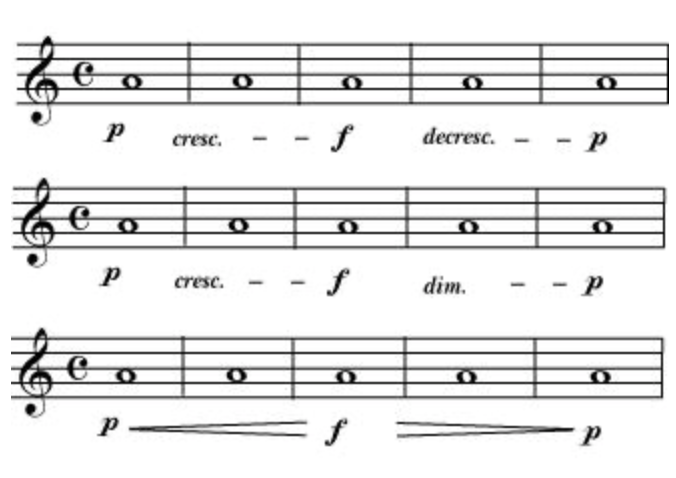
\includegraphics[width=0.5\textwidth]{/Users/leonardoangellotti/Desktop/tesi latex/immagini/dynamics} 
    \caption{simbolismo dinamiche in uno spartito}
    \label{fig:immagine}
\end{figure}

\subsection{scala armonica}

La scala maggiore è una delle scale diatoniche più comuni e ha un suono generalmente percepito come "felice" o "luminosa". \\
La scala maggiore segue uno schema specifico di toni (T) e semitoni (S). Lo schema è: \\
\texttt{T - T - S - T - T - T - S} \\
Ad esempio, la scala di Do maggiore (C maggiore) è: \\
\texttt{Do (C) - Re (D) - Mi (E) - Fa (F) - Sol (G) - La (A) - Si (B) - Do (C)} \\
\\
La scala minore ha un suono generalmente percepito come "triste" o "scuro".  \\
Segue uno schema diverso rispetto alla scala maggiore: \\
\texttt{T - S - T - T - S - T - T} \\
Ad esempio, la scala di La minore naturale (A minore naturale) è: \\
\texttt{La (A) - Si (B) - Do (C) - Re (D) - Mi (E) - Fa (F) - Sol (G) - La (A)} \\

\subsection{melodia}

Una melodia è una sequenza di note musicali che è percepita come un'unità singola e coerente. \\
Essa è una componente fondamentale della musica, essendo spesso la parte più riconoscibile di un brano musicale. \\
Una melodia è composta da una serie di note che vengono suonate in successione. Queste note possono variare in altezza (pitch), durata (rhythm), intensità (velocity). \\
Il \textbf{contorno melodico} si riferisce al profilo delle altezze delle note, ovvero come le altezze delle note salgono e scendono nel corso della melodia. Questo può includere salti, scale, ripetizioni e altre variazioni. \\
La melodia è spesso \textbf{basata su una scala musicale}, come una scala maggiore o minore, che fornisce un quadro armonico e tonale. 

\subsection{accordi}

Gli accordi sono combinazioni di tre o più note suonate simultaneamente o in sequenza arpeggiata, a creare un'armonia. \\
Gli accordi sono fondamentali nella musica, fornendo la struttura armonica su cui si basano melodie e progressioni. \\
Possono essere maggiori o minori, in base alla distanza tra le note. \\
\\
Un \textbf{problema fondamentale} nella generazione di musica tramite algoritmi, è la \textbf{scelta nella sequenza di una progressione di accordi}, che descrive lo stile musicale di una canzone e la sua \textit{orecchiabilità}. \\
\\
Esempi di Progressioni di Accordi usati comunemente in musica.\\
\\
Progressione \texttt{I-IV-V-I} in Do Maggiore: \\
Accordi: \texttt{Do (C) - Fa (F) - Sol (G) - Do (C)} \\
Uso comune nelle canzoni pop e rock (\textit{il giro di Do}) \\
\\
Progressione \texttt{ii-V-I} in Jazz: \\
Accordi: \texttt{Re min. settima (Dm7) - Sol settima (G7) - Do mag. settima (Cmaj7)} \\
Molto usata nel jazz per creare risoluzioni armoniche sofisticate.

\section{File MIDI}

Un file MIDI (Musical Instrument Digital Interface) è un formato di file standardizzato utilizzato per rappresentare \textbf{informazioni musicali in forma digitale}. \\
Invece di memorizzare il suono effettivo come fanno i file audio, un file MIDI memorizza i dati relativi alle note, agli strumenti, alle dinamiche e ad altre istruzioni musicali che possono essere riprodotte da dispositivi elettronici compatibili con il MIDI, come sintetizzatori, sequencer, computer e software di notazione musicale.

% Inserimento di un'immagine
\begin{figure}[H]
    \centering
    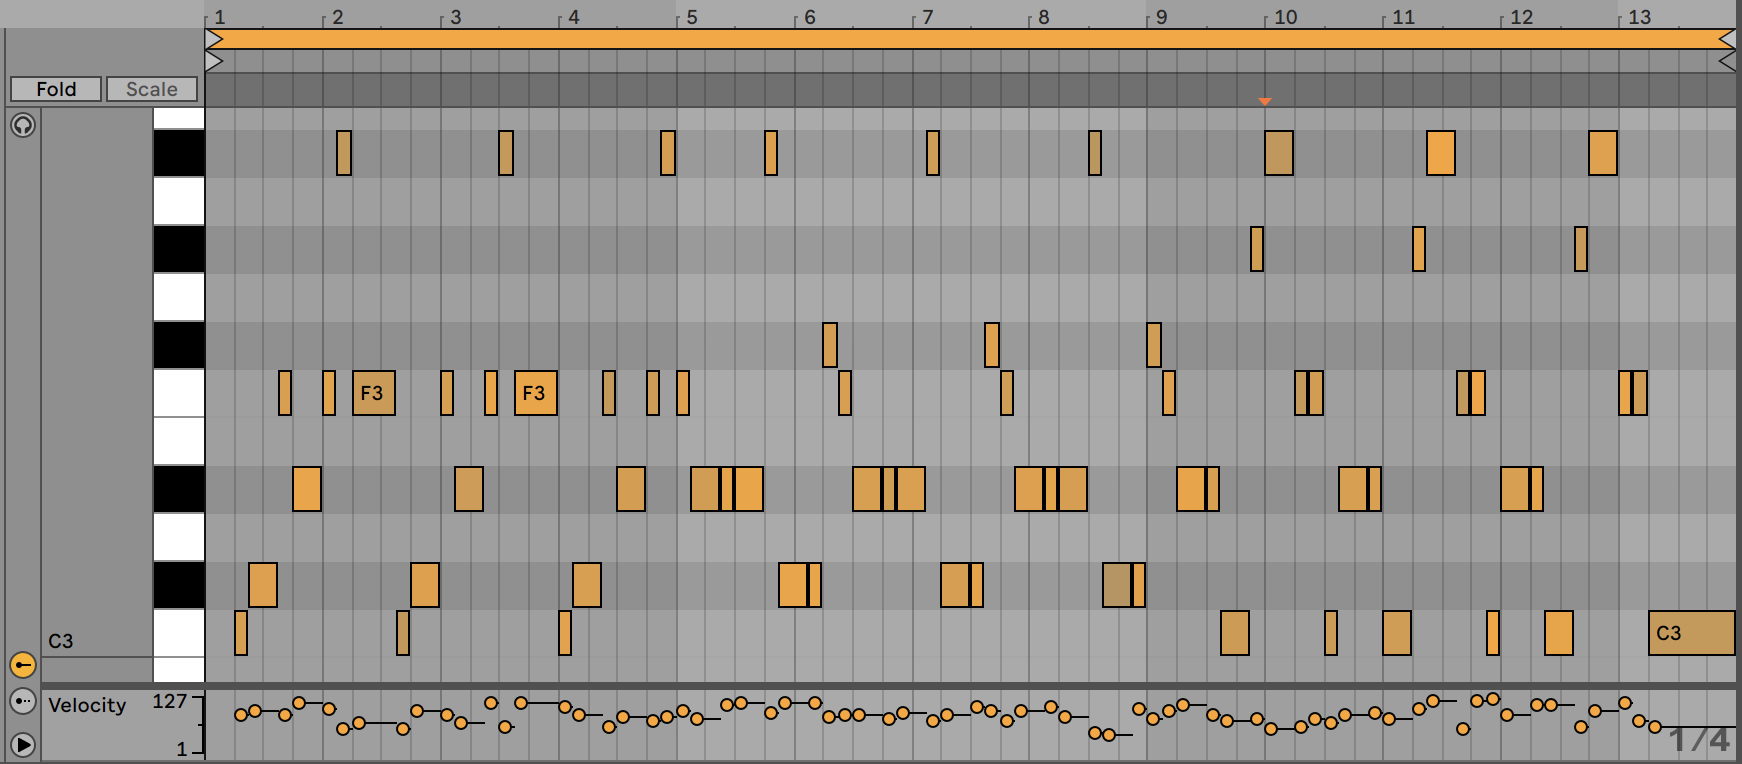
\includegraphics[width=1\textwidth]{/Users/leonardoangellotti/Desktop/tesi latex/immagini/midi} 
    \caption{esempio di un file midi importato in Ableton}
    \label{fig:immagine}
\end{figure}

\chapter{Metodi di generazione}

\section{generazione melodia}

Quando si considera il problema della generazione della musica, la forma più semplice di esercizio che viene in mente, è la composizione di \textbf{melodie monofoniche senza accompagnamento}.\\
Nella maggior parte dei sistemi di generazione le melodie vengono create con caratteristiche simili allo stile scelto.\\
Questi sistemi dipendono da una \textit{fitness-function} che valuta le sequenze generate.\\
Tale funzione di fitness è spesso basata sulla somiglianza con un determinato corpus, stile o brano, o dipende in generale dalle regole teoriche musicali.\\
\\
I primi tentativi di generare melodie con i computer risalgono al 1956, quando \textbf{Pinkerton} costruì un \textit{modello markoviano} , il \textbf{Banal Tune-Maker}, basato su un corpus di 39 semplici filastrocche, tuttavia il modello tendeva ad essere ripetitivo.\\
\\
Un altro problema nell'uso delle catene di Markov, risiede nell'eccessiva somiglianza con la melodia originale, e dunque nel plagio. \\
Il compromesso tra la composizione di brani simili a lavori esistenti, contro la necessità di doverne creare di nuovi e creativi, è difficile da ricercare. \\
Si ricorda a tal proposito una citazione di Stravinsky, celebre compositore Russo: \\
\textit{“i buoni compositori copiano, i grandi compositori rubano”}.\\
Riferendosi a quest'idea tuttavia le macchine non hanno ancora la capacità di distinguere tra il furto astuto e il plagio totale. \\
Con quest'intuizione è stata poi introdotta la variabile \textit{MaxOrder}, ad indicare il massimo ordine di sottosequenze simili consentito in una sequenza generata, con l'intento di limitare le ripetizioni eccessive nel materiale. \\
Esistono diverse tipologie di tali vincoli di controllo, ad esempio la volontà che una sequenza sia globalmente ascendente o che segua invece un intorno di note arbitrario. \\
\\
\textbf{Davismoon ed Eccles} (2010) sono stati alcuni dei primi ricercatori a inquadrare la generazione musicale come un problema di ottimizzazione combinatoria con un modello di Markov.  \\
Per valutare la musica generata, il loro sistema costruisce un secondo modello di Markov, riducendo poi al minimo la distanza euclidea tra il modello originale e il nuovo modello.  \\
Per risolvere questo problema di minimizzazione è stato utilizzato un processo di \textit{simulated-anealing}. \\
\\
Comporre una melodia monofonica può sembrare un compito semplice rispetto alla partitura di un'intera sinfonia. \\
Tuttavia, le melodie sono più che semplici movimenti tra le note, normalmente possiedono una \textbf{struttura a lungo termine}. \\
Negli ultimi anni, alcune ricerche hanno dimostrato l’efficacia dell’utilizzo di tecniche come il \textbf{deep learning} per rafforzare una consecuzione coerente. \\
\\
\textbf{Horner e Goldberg} (1991), pionieri nell'applicazione degli algoritmi genetici nella composizione musicale, affrontano il problema del \textbf{interpolazione tematica}, ovvero la trasformazione di un pattern musicale iniziale in uno finale, durante una durata specificata. \\
È stato creato un insieme (chiamato popolazione) di soluzioni iniziali, che attraverso una combinazione simile a quella genetica, ne ha generate di nuove. \\
\\
Sebbene esista molto lavoro sulla generazione di accordi data una melodia, alcuni studi si concentrano viceversa, sulla generazione di una melodia che si adatti a una sequenza di accordi. \\
\\
\textbf{Moorer} (1972), ad esempio, genera prima una sequenza di accordi, e successivamente una linea melodica su questa. \\
Le note della melodia sono limitate solo a quelle dell'accordo corrispondente in un dato momento. \\
Ad ogni punto si decide, sulla base di un modello markoviano, di invertire i frammenti melodici basati sull'accordo, oppure di copiarne da quello precedente. \\
Le brevi melodie risultanti tuttavia hanno un suono estraneo, ciò è legato al fatto che l'approccio melodico, non è quello utilizzato dagli esseri umani, infatti il sistema non discrimina le sequenze \textit{gradevoli}  da quelle \textit{non familiari}. 

\subsection{armonia}

L'armonia è definita da una relazione verticale tra note, che suonano contemporaneamente, e orizzontale, la relazione delle note nel tempo. \\
Il sistema deve generare sequenze riconoscibili nel genere musicale, o con la musica di un particolare artista, senza però mai essere \textit{sostanzialmente uguali} a gli esempi di riferimento. \\
\\
La maggior parte degli studi adotta approcci basati sul training-set per determinare possibili accordi in un dato segmento melodico, e garantire una corretta transizione tra questi, creando dapprima uno scheletro melodico. \\
\\
\textbf{Steedman} (1984) ha studiato melodie blues con lunghezza di 12 battute, definendo un piccolo insieme di regole, riuscendo a produrre le progressioni di accordi tipiche dello stile. \\
\\
\textbf{Lee e Jang} (2004) hanno utilizzato il modello di Markov, integrato con programmazione dinamica, per determinare il pattern armonico di una melodia canticchiata dall'utente; \\
le probabilità nella matrice di transizione tra le note correnti sono state apprese da un set di 150 canzoni. \\
\\
\textbf{Simon} (2008) ha adottato un approccio simile; allenando il proprio sistema su 298 brani di vari generi come jazz, rock, pop, blues e altri. \\
\\
Entrambi i sistemi vengono valutati tramite \textbf{feedback soggettivo}, cioè da un umano e non da una qualche fitness-function, a seguito di sessioni d'ascolto. \\
Uno svantaggio di questo approccio è che le sequenze di accordi generate tendono ad essere \textbf{generiche e indistinte nello stile}. \\
\\
Indipendentemente dalla rappresentazione utilizzata, la valutazione della musica è spesso un compito soggettivo e, come tale, una misura di fitness affidabile e solida può essere difficile da definire. \\
Molti dei primi ricercatori aggirarono questo problema impiegando l'uso di un giudice umano, e tali sistemi sono noti come \textbf{Interactive EC} (IEC). \\
Una funzione di fitness basata sull’uomo era stata precedentemente utilizzata con successo nell’evoluzione delle immagini, 
ma gli autori hanno notato una differenza pratica: \\
più immagini possono essere visualizzate contemporaneamente, e molto rapidamente, 
mentre la musica è un fenomeno temporale, e quindi tutti gli individui devono essere ascoltati in sequenza, uno dopo l'altro. \\
Ciò si traduce in un costo molto elevato nell’utilizzo di un essere umano come funzione di fitness. 

\subsection{ritmo}

Nei sistemi di generazione musicale il ritmo dipende dalla durata di ciascuna nota. \\
In generale, esistono meno sistemi di \textit{generazione ritmica} rispetto ai sistemi melodici. \\
\\
\textbf{Tokui e Iba} (2000) hanno proposto il sistema CONGA, che usa algoritmi genetici per produrre modelli ritmici, usando l'utente umano come funzione fitness. \\
Brevi frammenti di schemi ritmici formano gli elementi cromosomici nell'algoritmo; subendo poi trasformazioni come il crossover e mutazioni. \\
\\
Un algoritmo genetico è stato implementato anche da \textbf{Ariza} (2002), generando ritmiche derivanti da variazioni genetiche. \\
La funzione fitness è consistita nel calcolare la distanza tra il ritmo generato e l'originale, fornito dall'utente, attraverso differenti misure di distanza. 

\section{Algoritmo Genetico}

\subsection{musica evolutiva}

L'applicazione dei metodi di \textit{computazione evolutiva} nel campo musicale ha cominciato ad emergere all'inizio degli anni '90. \\
Ci sono tre criteri fondamentali da considerare: \\
\textit{il domino del problema,} \\
\textit{la rappresentazione individuale} \\
\textit{e la misura dell'idoneità}. \\
\\
Nella ricerca è fondamentale la codifica del dominio, e quindi i limiti o lo stile musicale, entro cui l'algoritmo ricerca. \\
Si definisce esattamente quale tipo di \textit{musica} si desidera sviluppare; si è intenzionati a creare melodie, armonizzazioni o progressioni di accordi? \\
\\
Nella rappresentazione individuale ci si chiede come rappresentare la musica: audio, spartiti stampati, messaggi MIDI? \\
comunemente, per una più facile gestione dei dati, si ricorre al formato MIDI, dove il genoma contiene valori di pitch e durate. \\
\\
Infine la questione della misura di idoneità: supponendo che due individui rappresentino brani musicali nel dominio desiderato, cosa rende uno “migliore” dell’altro? 

\subsection{Prime applicazioni dell'EC alla musica}

\textbf{Horner e Goldberg} furono tra i primi ad applicare un algoritmo genetico al processo di composizione musicale considerando il problema della \textit{transizione tematica}. \\
È stata considerata la trasformazione di una frase melodica in un'altra, dove i genomi rappresentavano la serie di transizioni necessarie.  \\
La fitness-function misurava quanto bene il modello finale corrispondesse al modello desiderato. \\
Il sistema tuttavia è stato utilizzato per creare \textit{transizioni}, piuttosto di creare effettivamente nuova musica. \\
\\
\textbf{John Biles} ha creato il sistema GenJam che utilizza un algoritmo genetico per evolvere gli assoli jazz. \\
GenJam ha utilizzato due popolazioni indipendenti: una per le misure di fitness ed una per la generazione di sequenze. \\
L’utente ha valutato queste frasi \textbf{in tempo reale} come \textit{buone} o \textit{cattive}. \\
Il sistema ha quindi utilizzato l'intero aggregato di frasi e misure per costruire un assolo jazz.

% Inserimento di un'immagine
\begin{figure}[H]
    \centering
    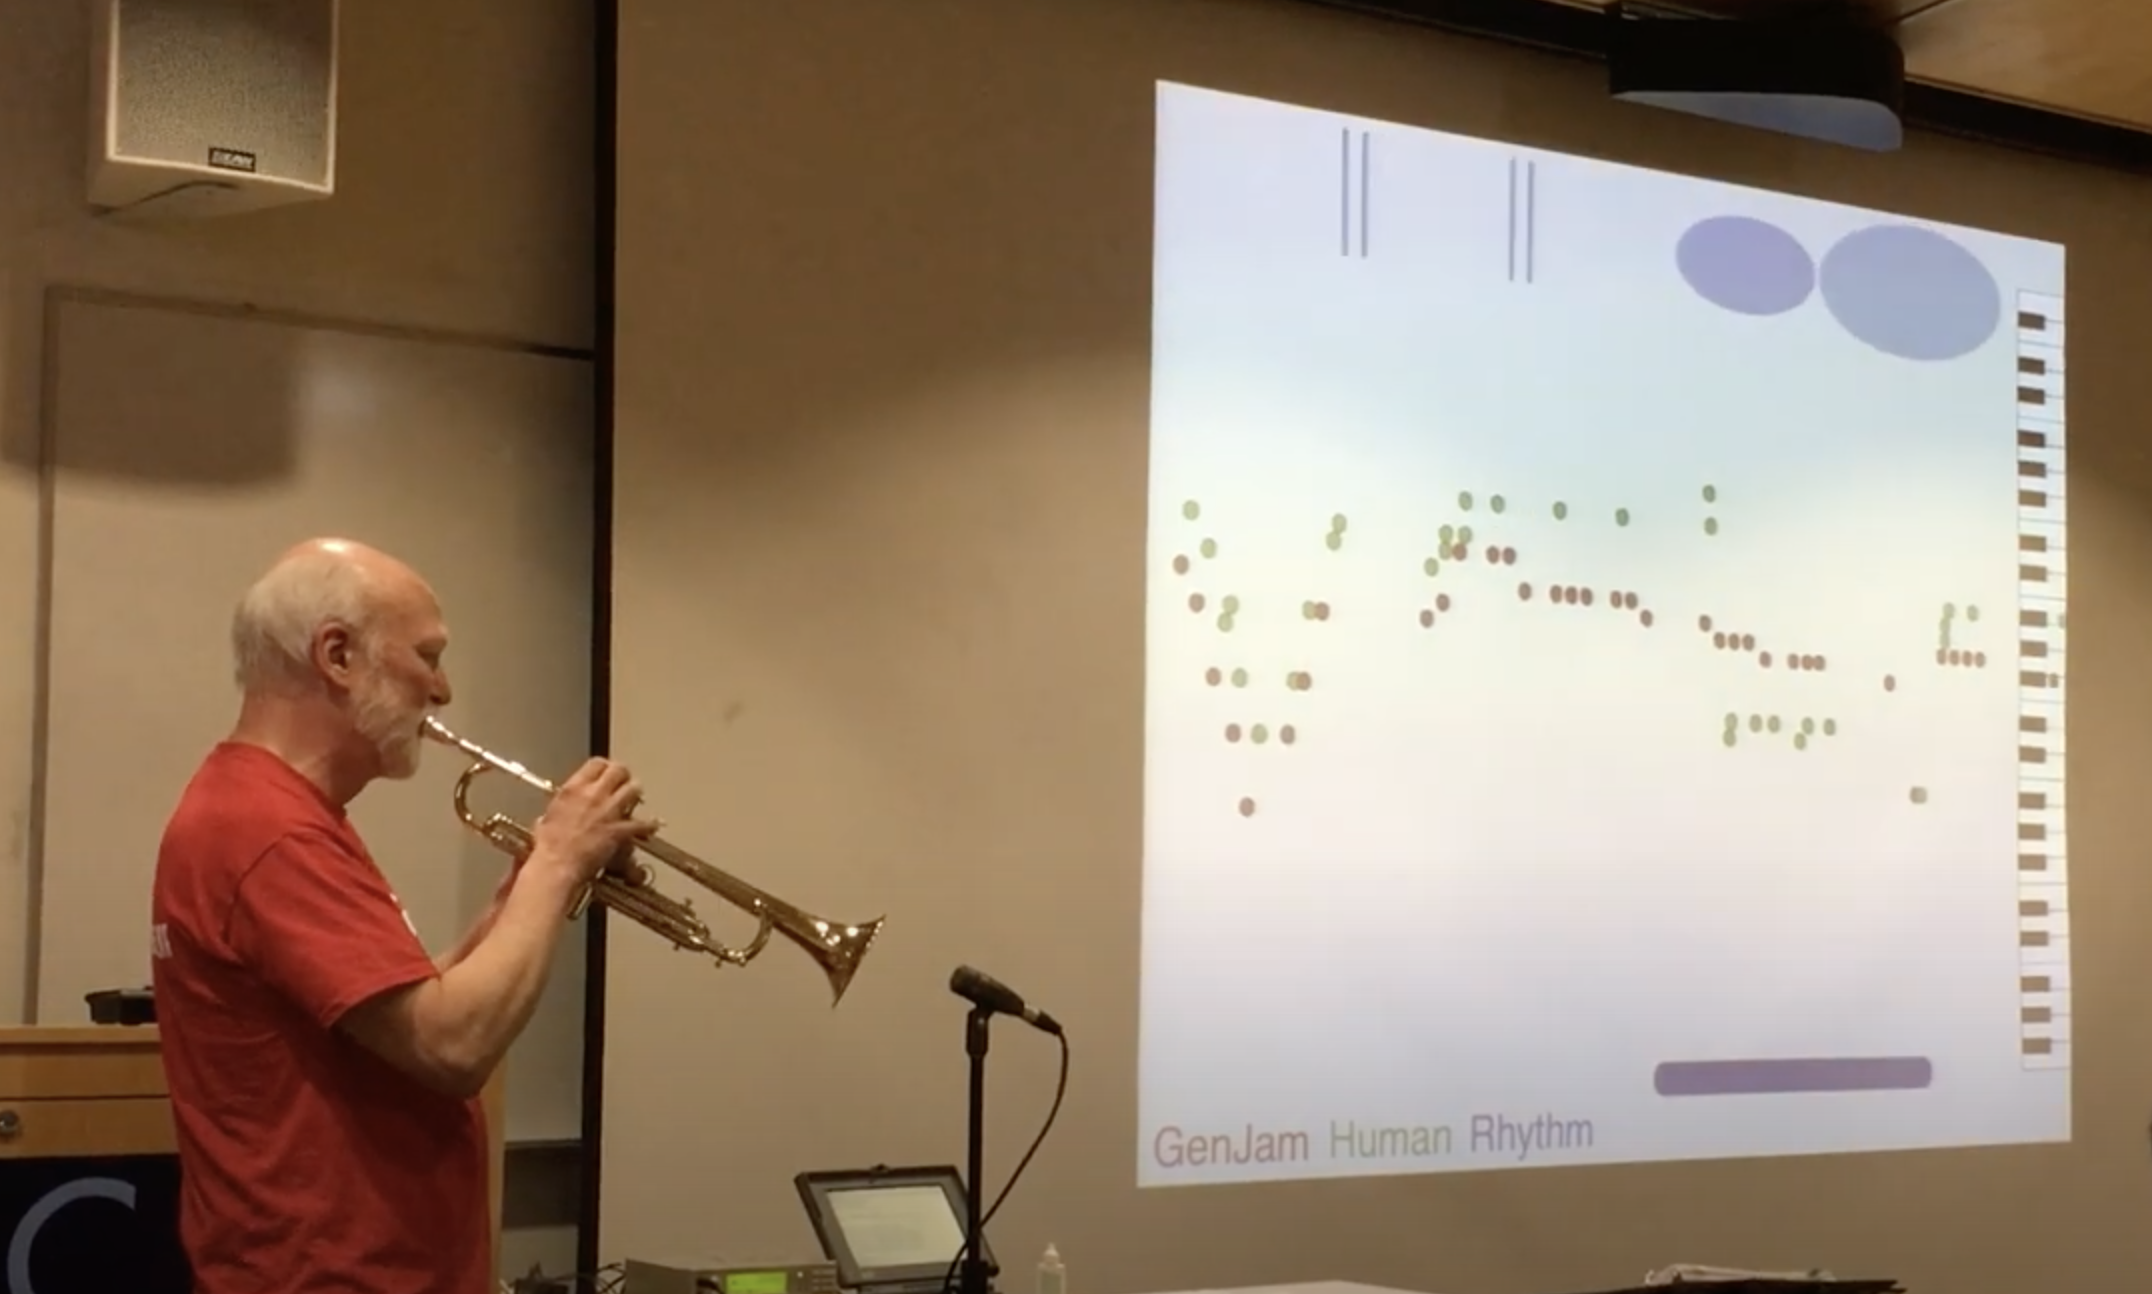
\includegraphics[width=1\textwidth]{/Users/leonardoangellotti/Desktop/tesi latex/immagini/GenJam} 
    \caption{John Biles suona assieme a GenJam}
    \label{fig:immagine}
\end{figure}

In studi successivi, si è \textbf{addestrata una ANN a fungere da funzione di fitness}, eliminando così la necessità dell'ascoltatore umano. \\
Tuttavia, in questo caso è riscontrato che i \textbf{risultati erano in qualche modo carenti} e si è stabilito che gli esseri umani ascoltano e sperimentano la musica in modi complessi e sottili, che non possono percepiti da modelli statistici come le ANN. \\

Negli studi che hanno fatto uso di ANN come fitness-function, gli autori hanno limitato il loro dominio, considerando solo armonie basate su tre accordi nella tonalità di Do maggiore, e creando solo melodie di quattro battute di durata. \\
La composizione è stata poi suddivisa in blocchi, e per ciascuno di questi un algoritmo genetico ha generato una popolazione.
Una ANN addestrata precedentemente da esempi forniti dall'utente, ha quindi giudicato i genomi candidati. \\
Gli autori hanno riconosciuto che questa combinazione di alg. gen. e ANN potrebbe produrre delle pseudo composizioni, 
ma le restrizioni applicate al dominio di addestramento hanno limitato fortemente il modello. \\
\\
Durante gli anni ’90 molti professionisti hanno applicato gli alg. gen. ad aspetti della generazione musicale, ma nessun metodo è risultato \textit{ideale} rispetto ad altri. \\
Gli esperimenti che utilizzano un corpus musicale per ricavare una misura di fitness saranno sempre limitati dal dominio scelto, limitando così il potenziale creativo del sistema. \\
Indipendentemente da quanto complessa o sfaccettata sia una data misura di fitness, è sicuramente \textit{impossibile dire che questa sia la misura definitiva della musica}. 

\section{L-System}

Gli L-system (o Lindenmayer system) sono un tipo di sistema formale utilizzato per modellare la crescita di \textit{piante ricorsive}. \\
Sono stati introdotti da Aristid Lindenmayer nel 1968 e sono composti da un alfabeto di simboli che, usati come insieme di regole di produzione, vengono impiegati per generare stringhe, a loro volta contenenti altri simboli, applicando appunto un approccio ricorsivo. \\
È necessario un assioma da cui iniziare, e meccanismi per interpretare le stringhe generate come strutture geometriche o altre forme di output. \\
\\
\textbf{Alfabeto:} I simboli dell'alfabeto possono rappresentare note musicali, durate, dinamiche, articolazioni, e altri elementi musicali. \\
\\
\textbf{Assioma:} La stringa iniziale può essere una sequenza di note. \\
\\
\textbf{Le regole} descrivono come trasformare ogni simbolo in una nuova sequenza di simboli musicali. \\
\\
Alfabeto: {A, B} \\
Assioma: A \\
Regole di produzione: \\
  \texttt{A → AB} \\
  \texttt{B → A} \\
\\
In questo esempio: \\
1. Partiamo dall'assioma \texttt{A}. \\
2. Applichiamo le regole: \\
    \texttt{A} diventa \texttt{AB} \\
   \texttt{AB} diventa \texttt{ABA} \\
   \texttt{ABA} diventa \texttt{ABAAB} \\
   e così via. \\
\\
Ora, mappiamo i simboli alle note musicali: \\
\texttt{A = Do} \\
\texttt{B = Re} \\
\\
La sequenza generata può essere interpretata come una melodia: \texttt{Do, Do-Re, Do-Re-Do, Do-Re-Do-Do-Re}, e così via. \\
\\
Gli L-system così permettono di generare pattern musicali ricorsivi e auto-simili che possono essere sia prevedibili che ma anche variabili. \\
\\
Nel paper \textit{Growing music}, \textbf{Peter Worth e Susan Stepney}, hanno sperimentato in modo più approfondito questo sistema. \\

Gli L-System permettono una maggiore sensibilità per il \textit{contesto}, cioè il rapporto tra le note lungo la sequenza, 
facendo crescere conseguentemente la pianta in modo diverso in base a gli elementi nell'intorno. \\
Questo potrebbe essere utile in musica, quando ad esempio il pezzo generato potrebbe raggiungere un climax o interrompersi bruscamente. \\
Per far ciò che questo avvenga, la regola di produzione per un L-System viene applicata al simbolo solo se compare inclusa ad altri simboli specifici. \\
La notazione \texttt{A < B > C} indica che agisce se la stringa \texttt{B} è presente con \texttt{A} alla sinistra e \texttt{C} a destra. \\
Viene considerato il seguente L-System \textit{sensibile al contesto}: 

% Inserimento di un'immagine
\begin{figure}[H]
    \centering
    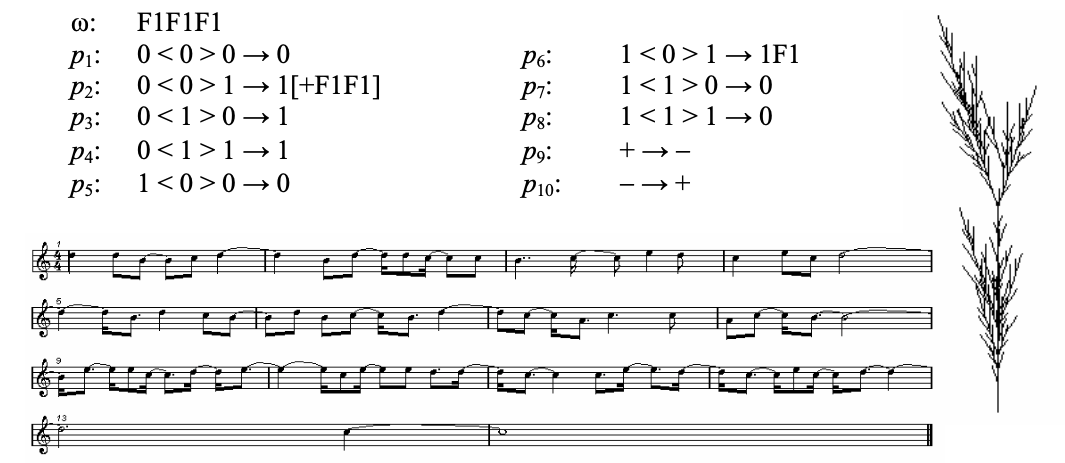
\includegraphics[width=1\textwidth]{/Users/leonardoangellotti/Desktop/tesi latex/immagini/L-system} 
    \caption{Descrizione dell'immagine}
    \label{fig:immagine}
\end{figure}

Questa melodia, e altre derivate in modo simile, suonano abbastanza \textit{casuali}; ricordano un assolo jazz. \\
Le note non rientrano bene nella cadenza 4/4 in una partitura, perché molte hanno una durata irregolare. \\
Tuttavia la melodia ritorna sempre a un motivo o una frase principale, a volte trasposto o suonato in un punto diverso della battuta. \\
Ad esempio, nella partitura sopra, una serie di note nella prima battuta è ripetuta nella nona battuta, ma in un modo insolito (trasposto in avanti per un quarto di tempo) e aumentate di 2 semitoni. \\
Questo tipo di simmetria rispecchia la musica normalmente composta o improvvisata, ed è dovuta dal tipo di struttura ricorsiva ad albero. 

\chapter{Progetto di musica genetica}

Viene ora introdotto un progetto di algoritmo genetico utile ad esemplificare fin quanto detto. \\
All'interno del progetto la funzione:

% Inserimento di un esempio di codice
\begin{lstlisting}[language=Python]
 
# Main function for running all helper functions and handling user input.
def genetic_algorithm(key, root, tempo, rythm):

\end{lstlisting}

scrive su disco 10 genotipi di sequenze di note, in formato MIDI, come risultato dell'esecuzione dell'algoritmo genetico. \\
La funzione prende in input dall'utente \\
\textbf{la scala} (key) utilizzata nella scelta delle note, può essere \textit{major} o \textit{minor}. \\
\textbf{La nota fondamentale} che indica la tonalità della canzone (root), e sulla quale verrà costruita la scala (es: \texttt{C, C#, D, D#, E, F, F#, G, G#, A, A#, B}) \\
\textbf{Il numero di battiti al minuto} (bpm), ovvero la velocità di esecuzione, della composizione \\
\textbf{il ritmo della composizione}, ovvero la durata delle note, a scelta tra quattro predefiniti (\textit{rock, jazz, dance, bossa nova}). \\
\\
All'interno della funzione troviamo 

\begin{lstlisting}[language=Python]

    # Build the scale based on the root note and chosen scale type
    scale = buildScale(root, key)

\end{lstlisting}

Restituisce un array, dove ogni numero rappresenta il codice MIDI di ogni nota. \\
L'array rappresenta la scala, maggiore o minore, costruita partendo dalla nota fondamentale scelta. \\
Viene eseguita poi l'evoluzione vera e propria, attraverso la crescita del genoma.

\subsection{Run-Evolution}

\begin{lstlisting}[language=Python]

    # Run the genetic algorithm to evolve a melody using the specified mutation rate and scale
    evolvedMelody = runEvolution(MUTATION_RATE, scale)

\end{lstlisting}

\texttt{runEvolution} implementa un algoritmo genetico che migliora in modo iterativo la popolazione di genomi musicali attraverso selezione, crossover e mutazione, l'esecuzione avviene finché non viene raggiunto un genoma con il punteggio \texttt{MAX-FITNESS} specificato. \\
Viene inizialmente creata un popolazione, inizializzata con metodo random. La popolazione è composta da 10 genomi. \\
Ogni genoma è un elenco di 8 battute, ciascuna contenente 8 note, tutte scelte casualmente dalla scala specificata. \\
Il codice che segue rappresenta lo sviluppo dell'algoritmo genetico utilizzato.

\begin{lstlisting}[language=Python]

 # Iterate for a maximum number of generations
    for _ in range(MAX_GENERATIONS):

        # Sort the population based on fitness scores in descending order
        population = sorted(population, key=fitnessFunction, reverse=True)
        
        # Select the top 2 genomes (the fittest) to carry over to the next generation
        nextGeneration = population[:2]

        # Generate the rest of the next generation through crossover and mutation
        for _ in range(len(population) // 2 - 1):

            # Select two parent genomes based on their fitness
            parentA, parentB = selectParents(population)
            # Perform crossover to produce two child genomes
            childA, childB = multipointCrossover(parentA, parentB)
            # Mutate the child genomes and add them to the next generation
            nextGeneration += [mutateGenome(childA, mutationRate, scale), mutateGenome(childB, mutationRate, scale)]

        # Update the population with the new generation
        population = nextGeneration
        
\end{lstlisting}

Per un numero massimo di generazioni prefissato, vengono create popolazioni di genomi. \\
Successivamente alla prima inizializzazione randomica, viene applicata la Fitness-Function, che assegna ad ogni genoma un peso/punteggio basandosi sui propri criteri di valutazione (vedremo in seguito). \\
Nella successiva popolazione vengono mantenuti i primi due genomi con il punteggio più alto, mentre per i restanti 8 vengono selezionati di volta in volta due genitori, da cui attraverso un (multipoint) crossover danno luogo a due figli, i quali subiscono una fase di mutazione. \\
I processi di crossover e mutazione sono definiti di \textit{exploration}, perché servono ad esplorare soluzioni che i due migliori genomi non sono riusciti ad ottenere. \\
Viceversa i due genomi mantenuti con il punteggio più alto, che si tramandano da una popolazione alla successiva, servono a garantire la migliore performance ad ogni generazione, qualora i genomi di exploration non diano risultati soddisfacenti. \\
Quando avviene che in una popolazione, i figli generati ottengano un punteggio superiore ai due migliori correnti, questi vengono dunque sostituiti. \\
Al termine del numero massimo di generazioni (prefissato, \texttt{MAX-GENERATIONS}), viene scritta su disco l'ultima popolazione costituita da 10 genomi. \\
Il migliore tra questi (con punteggio più alto) viene chiamato \texttt{best-genome.mid}. 

\subsection{fitness-function}

La fitness function calcola il punteggio finale ponderando e sommando i punteggi dei componenti per \textbf{fluidità, ritmo e armonia}, restituendo il risultato. \\
Vengono inizializzati i pesi e i punteggi.

\begin{lstlisting}[language=Python]

 # Weights for the different fitness components
    smoothnessWeight = 15
    restWeight = 5
    harmonyWeight = 20

    # Initialize fitness scores
    smoothnessScore = 0
    restScore = 0
    harmonyScore = 0
    
\end{lstlisting}

L'harmonyscore riporta il punteggio di armonizzazione tra le note, ovvero come queste suonino \textit{bene} tra loro. \\
Di seguito un dizionario in cui troviamo come chiave, la distanza tra la nota corrente e la precedente, e come valore, il punteggio assegnato a tale distanza armonica.

\begin{lstlisting}[language=Python]

    # Harmony intervals table for scoring harmony
    harmonyIntervalsTable = {
        0: -20, 1: 5, 2: 5, 3: 50, 4: 50, 5: 30, 6: -10, 7: 50, 8: 10, 9: 40, 10: -2, 11: -2, 12: 10,
        13: -5, 14: 5, 15: 5, 16: 50, 17: 50, 18: 30, 19: -10, 20: 50, 21: 10, 22: 40, 23: -2, 24: -2, 25: 10
    }

\end{lstlisting}

- Intervalli consonanti perfetti (0, 7, 12, 19, 24 semitoni): Questi intervalli, che corrispondono alle ottave e quinte perfette (e le loro ripetizioni all'ottava superiore), hanno punteggi molto alti (50 o 10), ad indicare di essere \textit{armoniosi}. \\
    - 0 (Unisono): 50 \\
    - 7 (Quinta giusta): 50 \\
    - 12 (Ottava giusta): 10 \\
    - 19 (Unisono all'ottava superiore): -10 \\
    - 24 (Due ottave giuste): 10 \\
\\
- Intervalli consonanti maggiori (4, 9, 16, 21 semitoni): Questi includono la terza maggiore e la sesta maggiore, che sono generalmente considerati molto armoniosi. \\
- Intervalli consonanti minori (3, 8, 17, 22 semitoni): Questi includono la terza minore e la sesta minore. \\
\\
- Intervalli dissonanti (1, 2, 6, 10, 11, 13, 23 semitoni): Questi includono la seconda minore, la settima minore e la settima maggiore, che sono considerati meno armoniosi o dissonanti. \\
    - 1 (Seconda minore): 5 \\
    - 2 (Seconda maggiore): 5 \\
    - 6 (Tritono): -10 \\
    - 10 (Settima minore): -2 \\
    - 11 (Settima maggiore): -2 \\
    - 13 (Ottava aumentata): -5 \\
    - 23 (Nona aumentata): -2 \\
\\
\textbf{Calcolo del punteggio di fluidità (\texttt{smoothnessScore})}: \\
Se la differenza tra le note (\texttt{noteDifference}) è 0 (unisono), il punteggio di fluidità viene diviso per 10, penalizzando fortemente la ripetizione della stessa nota. \\
Se la differenza è minore o uguale a 2 semitoni, aumenta il punteggio di fluidità di 1, incentivando piccoli movimenti tra le note. \\
Se la differenza è di 11 semitoni (quasi un'ottava), il punteggio di fluidità viene diviso per 2, penalizzando questo ampio intervallo. \\
Per altri intervalli, il punteggio di fluidità aumenta di \texttt{1 / oteDifference}, favorendo movimenti più piccoli tra le note. \\
Se \texttt{noteDifference} è 0, si evita la divisione per zero assegnando 0. \\
Il codice cerca dunque di bilanciare l'armonia (basata sugli intervalli predefiniti) e la fluidità (basata sulla distanza tra note consecutive) in una sequenza musicale, con vari meccanismi per favorire o penalizzare certi tipi di movimenti tra le note. 

\begin{lstlisting}[language=Python]

if note is None and prevNote is None:
    consecutiveRests += 1

\end{lstlisting}

Se entrambe note e \texttt{prevNote} sono \texttt{None}, significa che si è verificata una pausa consecutiva: Incrementa il contatore \texttt{consecutiveRests}.

\begin{lstlisting}[language=Python]

if numRests * 10 <= len(flatten(genome)):
    restScore += 10

\end{lstlisting}

Se il numero di pause (\texttt{numRests}) moltiplicato per 10 è inferiore o uguale alla lunghezza della sequenza musicale piatta (\texttt{flatten(genome)}), aumenta il punteggio ritmico (\texttt{restScore}) di 10. \\
Questo premia una quantità ragionevole di pause nel contesto della lunghezza totale del genoma musicale, suggerendo che alcune pause sono considerate musicalmente desiderabili.

\begin{lstlisting}[language=Python]

if consecutiveRests:
    restScore -= (consecutiveRests * 10)

\end{lstlisting}

Se ci sono pause consecutive (\texttt{consecutiveRests > 0}), penalizza il punteggio ritmico diminuendo \texttt{restScore} di \texttt{consecutiveRests * 10}. \\
Questo penalizza pesantemente le pause consecutive, suggerendo che una lunga serie di pause è considerata indesiderabile dal punto di vista ritmico.

\begin{lstlisting}[language=Python]

fitness_weight_genome = (smoothnessScore * smoothnessWeight) + (restScore * restWeight) + (harmonyScore * harmonyWeight)

\end{lstlisting}

Il punteggio di fitness finale (\texttt{fitness-weight-genome}) è calcolato come la somma ponderata dei punteggi componenti. \\
Ogni punteggio componente (\texttt{smoothnessScore, restScore, harmonyScore}) viene moltiplicato per il rispettivo peso (\texttt{smoothnessWeight, restWeight, harmonyWeight}). \\
La somma dei prodotti risultanti rappresenta il punteggio di fitness finale del genoma. \\
\\
I pesi (\texttt{smoothnessWeight, restWeight, harmonyWeight}) permettono di enfatizzare o de-enfatizzare specifici aspetti della valutazione a seconda degli obiettivi desiderati per la composizione musicale. \\
Ad esempio, aumentando il peso della fluidità, si darà maggiore importanza alle transizioni tra le note, mentre aumentando il peso dell'armonia, si enfatizzerà la qualità armonica della melodia. \\
Questo metodo di valutazione è utile in contesti come algoritmi genetici per la generazione di musica, dove è necessario valutare e selezionare sequenze musicali basate su criteri compositi.

\subsection{risultati}

Eseguiamo dunque il programma. \\
Sono riportati le opzioni scelte per una generazione musicale esemplificativa.

% Inserimento di un'immagine
\begin{figure}[H]
    \centering
    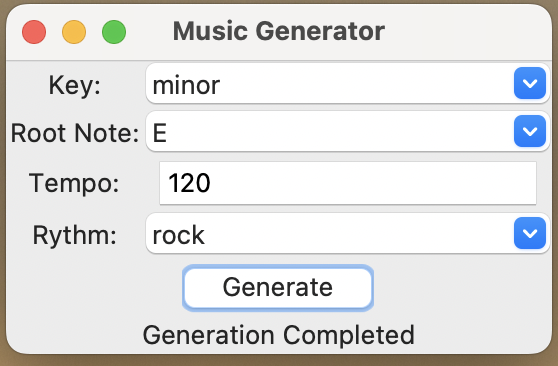
\includegraphics[width=0.5\textwidth]{/Users/leonardoangellotti/Desktop/università/terzo anno/tesi/MusicGeneticAlgorithm-main/genetic_music/final results rock/results/setting} 
    \label{fig:immagine}
\end{figure}

Al termine dell'esecuzione vengono stampati i risultati dei punteggi ottenuti dalla fitness function, per i genomi di ogni popolazione.

% Inserimento di un'immagine
\begin{figure}[H]
    \centering
    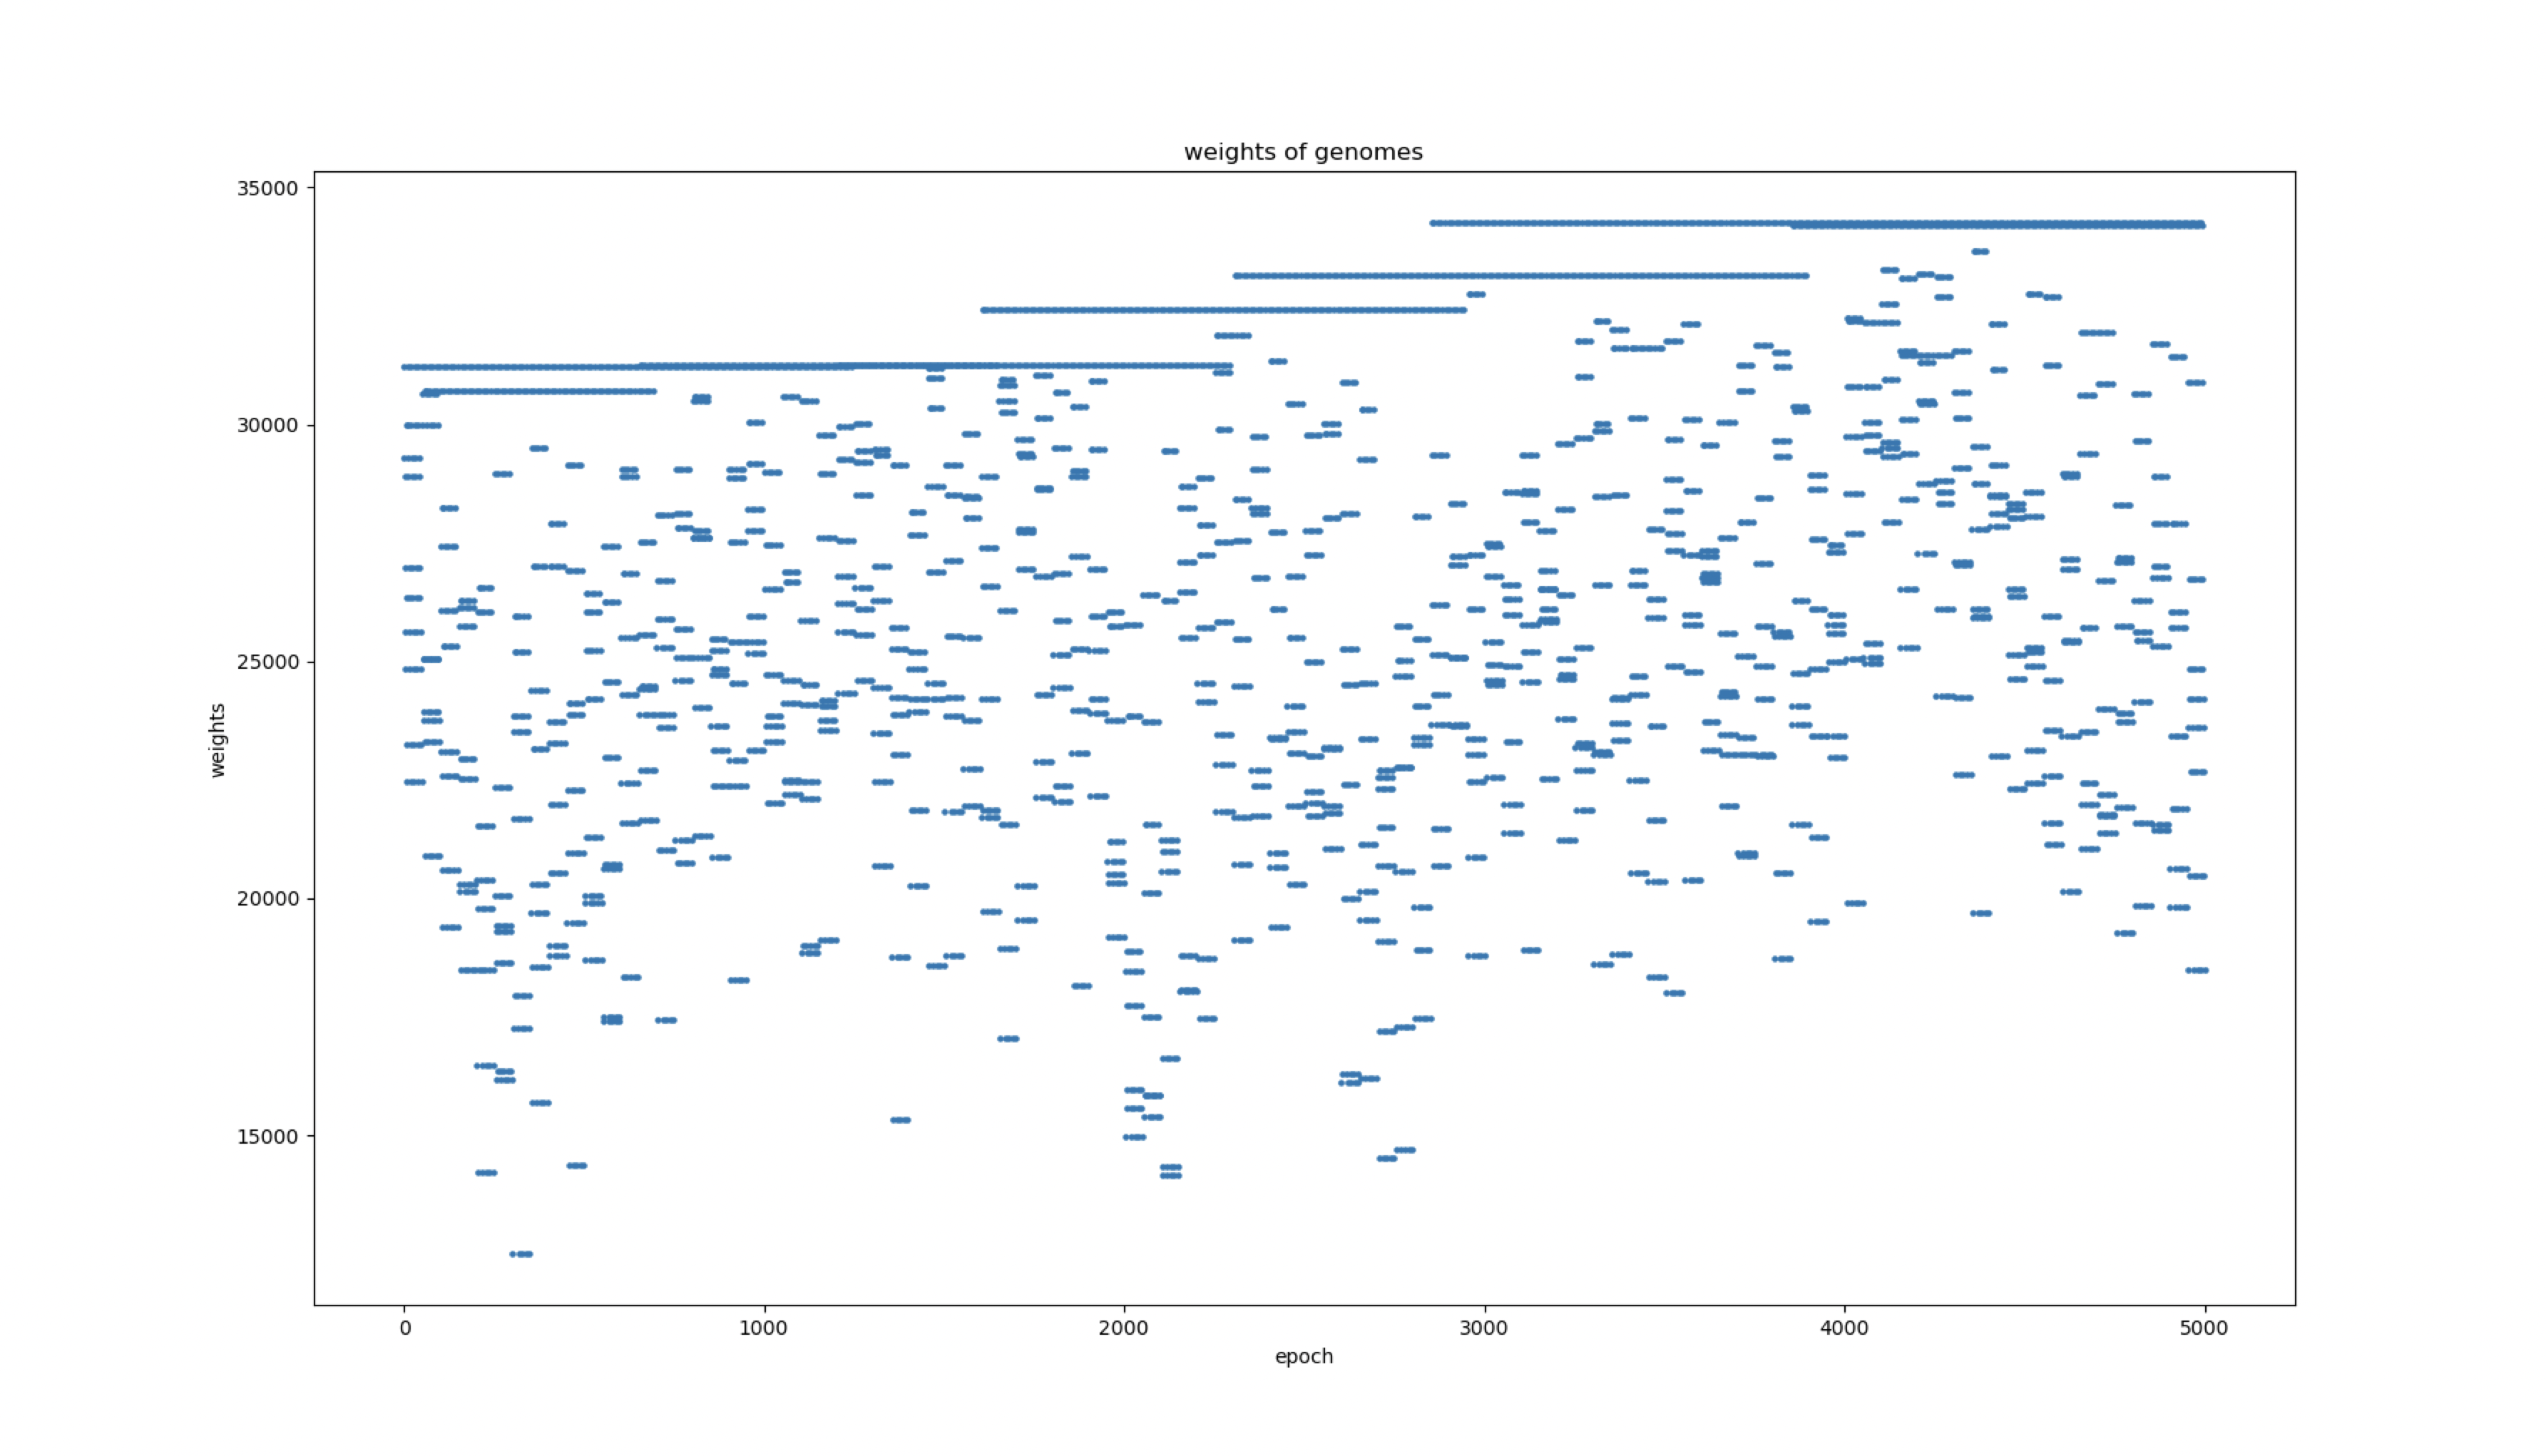
\includegraphics[width=1\textwidth]{/Users/leonardoangellotti/Desktop/università/terzo anno/tesi/MusicGeneticAlgorithm-main/genetic_music/final results rock/results/scores} 
    \label{fig:immagine}
\end{figure}

Le linee che si mantengono costanti sono i punteggi dei primi due genomi (con punteggio più alto ad ogni generazione) che nell'algoritmo scelto vengono tramandati senza alcuna alterazione (crossover, mutation). \\
Quando "nasce" un nuovo genoma che si verifica avere un punteggio più altro dei primi due, questo fissa un nuovo livello di punteggio superiore ai precedenti, che viene mantenuto finché ciò non accade nuovamente. \\
Questa procedura garantisce un costante aumento del punteggio e un conseguente miglioramento tra le popolazioni. \\
La nuvola di punti che appaiono al di sotto, con punteggio inferiore, appartengono al set di genomi soggetti a crossover e mutazioni. \\
Al termine della procedura evolutiva, vengono stampati i 10 genomi appartenenti all'ultima popolazione.

% Inserimento di un'immagine
\begin{figure}[H]
    \centering
    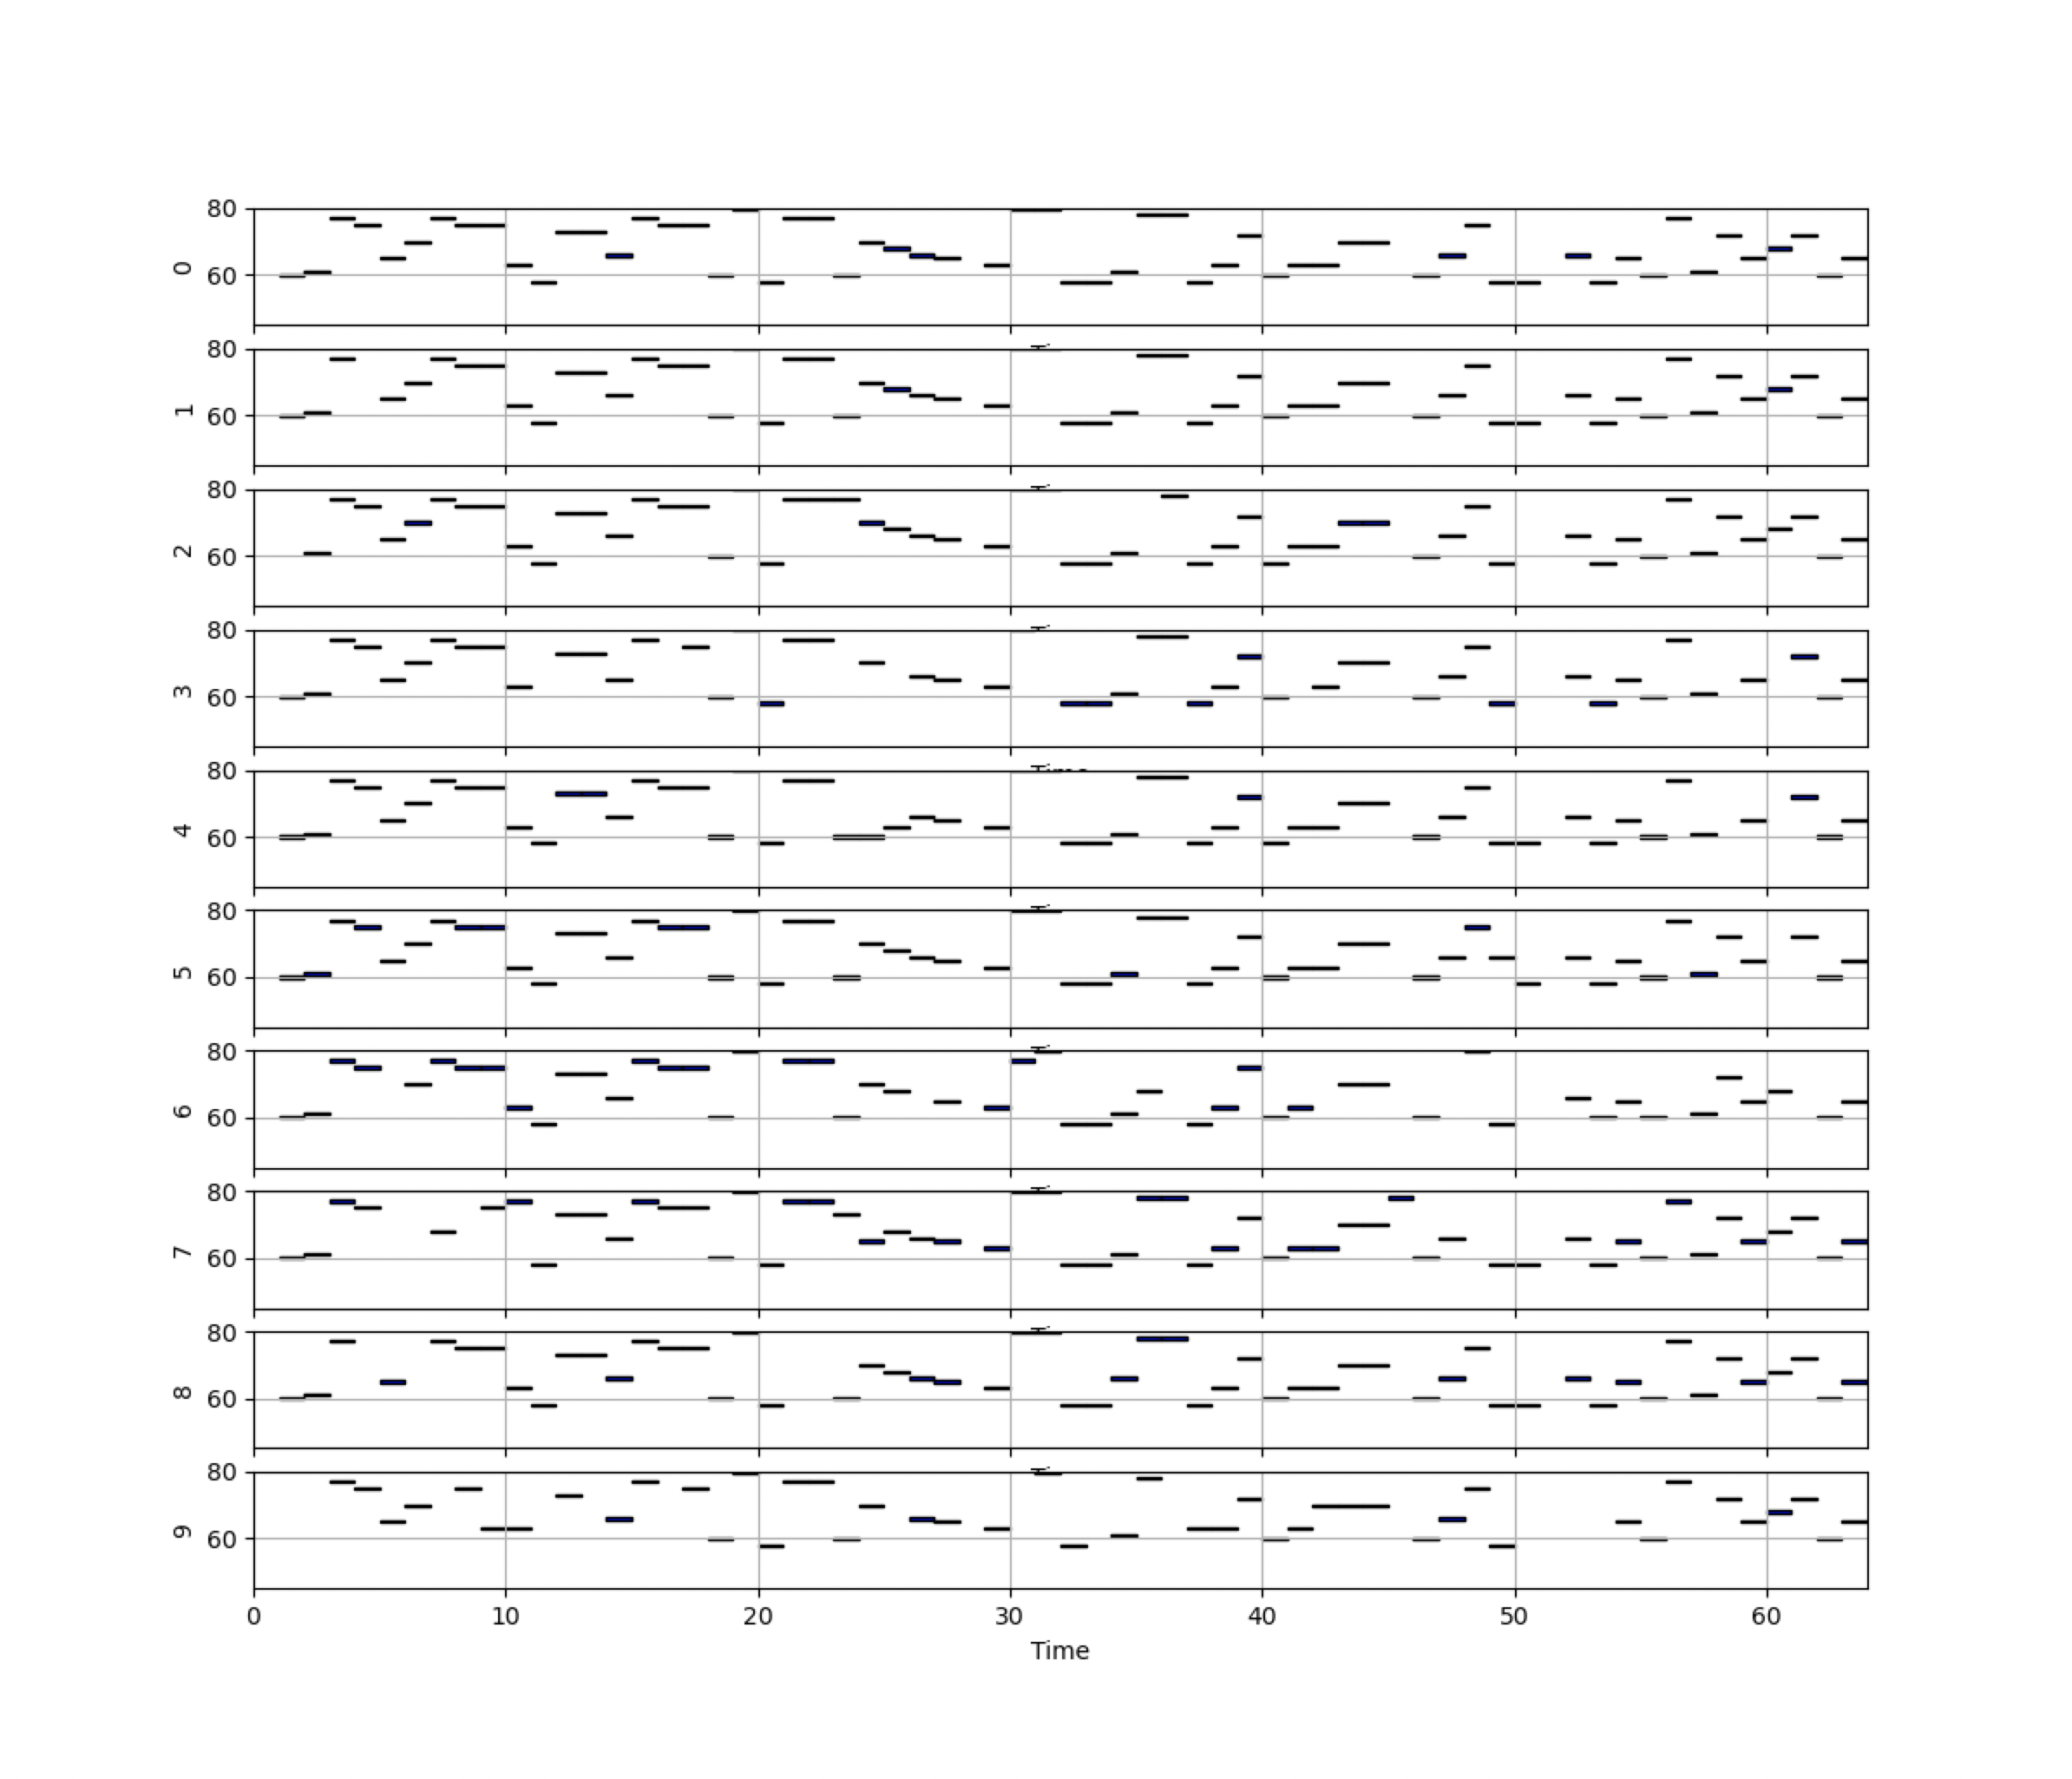
\includegraphics[width=1\textwidth]{/Users/leonardoangellotti/Desktop/università/terzo anno/tesi/MusicGeneticAlgorithm-main/genetic_music/final results rock/results/MIDI} 
    \label{fig:immagine}
\end{figure}

La stampa rappresenta 10 file midi, dal migliore (numero 0) al "peggiore" (numero 9) secondo la nostra fitness-function. \\
Le note sono rappresentate dalle linee orizzontali che appaiono a diverse altezze di pitch, indicati nell'asse delle ordinate. \\
Le note sono sequenziali, appaiono dunque in momenti consecutivi, con diversa durata (dettata dal ritmo scelto dall'utente). \\
Si ricorda che l'algoritmo genera una sequenza monofonica, infatti non appare più di una nota contemporaneamente. \\
Le sequenze vengono salvate su disco. \\
Il genoma migliore prende il nome di \texttt{best-genome.mid}, mentre ai restanti viene assegnato un numero in ordine decrescente in punteggio (\texttt{genome-0.mid}, ..., \texttt{genome-8.mid}). \\
\\
Ad un primo ascolto di \texttt{best-genome.mid}, percepiamo un movimento coerente nella teoria, ordinato nel ritmo, ma non regolare nel tempo. \\
Non viene percepita infatti alcuna vera struttura compositiva, questo perché la fitness function si è preoccupata di fare confronti solo tra una nota e la precedente, e non tra tutte le note della sequenza. \\
Non esiste dunque una vera struttura a lungo termine, una struttura narrativa, avente inizio svolgimento e fine, propria invece di qualsiasi genere musicale. \\
Non è presente nemmeno il classico schema delle canzoni pop: \textit{verso-ritornello-verso-ritornello-bridge-ritornello}. \\
\\
Per ovviare a questo difetto si procedere con un'operazione naive ma efficace: \\
Si decide di generare una nuova sequenza, chiamata \texttt{repeated-melody.mid}, la quale ripete per 4 volte le prime 3 bar prese dal \texttt{best-genome.mid}. \\
Il risultato risulta essere \textit{ripetitivo} e dunque intrinsecamente più regolare, oltre a essere per il nostro orecchio più confortevole. \\
\\
Abbiamo dunque ottenuto un risultato teorico \textit{accettabile} e \textit{coerente}. \\
Possiamo ottenere di più nella pratica? \\
Si. \\
Importando il file midi (\texttt{repeated-melody.mid}) in una DAW (Digital Audio Workstation, in questo caso è stato utilizzato Ableton) possiamo apportare ulteriori modifiche. \\
Viene assegnata alla traccia lo strumento \textit{Grand Piano}. \\
Su questa vengono applicate le seguenti opzioni

% Inserimento di un'immagine
\begin{figure}[H]
    \centering
    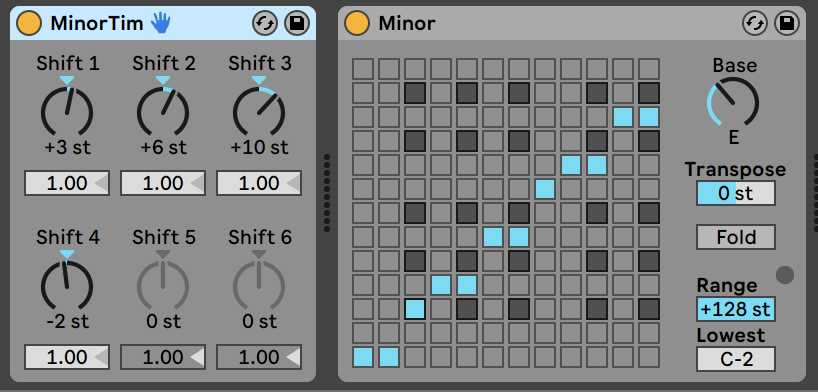
\includegraphics[width=0.6\textwidth]{/Users/leonardoangellotti/Desktop/università/terzo anno/tesi/MusicGeneticAlgorithm-main/genetic_music/final results rock/results/ableton_settings} 
    \label{fig:immagine}
\end{figure}

\textit{MinorTim} permette di generare più note, ad una certa distanza in semitoni, partendo dalla nota corrente. \\
Nel caso specifico un accordo minore. \\
Tuttavia un primo ascolto risulta essere poco piacevole, perché le note generate non considerano la scala di riferimento. \\
È necessario dunque usare lo strumento "Minor" per ancorare ogni nota in una posizione coerente. \\
Il risultato è decisamente più armonico, seppur tuttavia ancor troppo \texttt{piatto} con nessuna variazione nell'esecuzione. \\
Per far fronte a questa \texttt{freddezza} ed aumentare la dinamicità è possibile randomizzare, in modo automatico, i valori di Velocity nella sequenza per ciascuna nota. \\
Un nuovo ascolto ci ricorda un qualche compositore jazz, immerso nel suo fiume di sentimenti, vissuti istante per istante, 
ma che vuole comunque mantenere, per piacere della clientela, un ritmo e melodia regolari. \\
\\
Per rendere il risultato ancor più gradevole, e musicalmente completo, possiamo aggiungere un elemento di percussioni, come una batteria. \\
Per il risultato ottenuto è stato utilizzato il plug-in \href{https://magenta.tensorflow.org/studio}{Magenta}  sviluppato da Google e attualmente disponibile gratuitamente. \\
In particolare è stato utilizzata la funzione \texttt{Drumify}, che data una sequenza di note, genera un secondo file MIDI in cui, similmente per il piano, vengono indicate le parti della batteria da percuotere (piatto, charleston, gran cassa, rullante). \\
In particolare, nel risultato finale, quest'ultima sequenza MIDI è stata processata dal Plugin \href{https://www.toontrack.com/product/superior-drummer-3/?gad_source=1&gclid=Cj0KCQjws560BhCuARIsAHMqE0H2FsGI5sBj5JLtPNhhiKiLf9qMEccOntk8F9uc4_ZvSDPK5TCZZKUaAg1LEALw_wcB}{SuperiorDrummer3},
una libreria sofisticata che raccoglie suoni di batteria accurati. \\
Si vuole far notare, che l'algoritmo implementato in \texttt{Drumify}, si basa su una neural network, non è di tipo genetico come nel caso del nostro esempio, in grado dunque di cogliere e sviluppare una certa consequenzialità tra parti. \\
\\
Infine, per le basse frequenze è stata aggiunta una semplice linea di basso, trasponendo la melodia due ottave inferiori, eliminando a mano, secondo il propio gusto, le note ridondanti, lasciando invece quelle fondamentali e di maggiore durata. \\
Il risultato finale, nello specifico, è \textit{quasi accettabile}, considerando che per generarlo sono state necessarie poco più di 500 linee di codice (commenti inclusi) e qualche plugin dal mondo di internet. \\
Il tratto fondamentale risiede nel fatto che per ottenere questo file mp3, non abbiamo mai: né dovuto suonare un pianoforte, pizzicare un basso o ritmare una batteria a tempo. \\
\\
Si possono sperimentare ulteriori modifiche, cambiando i pesi (\texttt{smoothnessWeight, restWeight, harmonyWeight]) o implementando un sistema nell'assegnazione della durata e velocity nelle note, ora affidate ad array con valori prefissati (rock, jazz, dance, bossa nova) e ad una scelta random rispettivamente.

\chapter{Conclusioni}

Negli ultimi decenni, la ricerca sulla generazione musicale ha compiuto enormi progressi nella generazione di aspetti ben definiti della musica, come la melodia, l’armonia, il ritmo e il timbro. \\
Modelli statistici all’avanguardia, tecniche di ottimizzazione avanzate, database digitali più grandi su cui addestrare i modelli e l’aumento della potenza di calcolo hanno portato alla produzione di sistemi migliori. \\
\\
Perché allora non utilizziamo sistemi di generazione musicale nella nostra vita quotidiana? \\
\\
L’indagine di cui sopra mostra che rimane un’importante sfida generale: quella di creare musica con una struttura a lungo termine. \\
La struttura a lungo termine, che spesso assume la forma di temi, motivi e schemi ricorrenti, è una parte essenziale di qualsiasi esperienza di ascolto musicale. \\
Per rendere i sistemi musicali generati dal computer parte della nostra vita quotidiana, c’è bisogno di sistemi più “narrativi", in grado cioè di creare un inizio, sviluppo e conclusione nella musica. \\
Sebbene ci siano recenti tentativi di generare musica con tensione [Farbood et al. 2007; Herremans e Chew 2016a], che sia applicata a colonne per videogiochi o che accompagnano film, c’è ancora margine di miglioramento per comprendere meglio la connessione tra musica ed emozione. \\
Sebbene le tecniche di apprendimento automatico possano essere estremamente efficaci, di solito richiedono grandi quantità di dati. \\
Esiste un potenziale reale affinché il lavoro futuro si sposti verso sistemi intelligenti che non richiedano abbondanti quantità di tracce audio, o sequenze musicali, 
capaci cioè di un ragionamento innato, rispecchiando meglio il funzionamento della mente umana. \\
Ciò risolverebbe anche la continua sfida di trovare un equilibrio tra la rigenerazione della musica esistente, o frammenti di questa senza ricadere nel plagio.

\appendix
\chapter{Appendice A}
\section{Dettagli aggiuntivi}

\chapter{Appendice B}
\section{Altro materiale supplementare}

% Esempio di citazione
Come descritto da Lamport \cite{latex}, e come discusso da Doe e Smith \cite{example_article}, i metodi utilizzati sono basati su...

% Bibliografia
\bibliographystyle{plain}
\bibliography{bibliografia}

\end{document}
